%iffalse
\let\negmedspace\undefined
\let\negthickspace\undefined
\documentclass[journal,12pt,onecolumn]{IEEEtran}
\usepackage{cite}
\usepackage{amsmath,amssymb,amsfonts,amsthm}
\usepackage{algorithmic}
\usepackage{graphicx}
\usepackage{textcomp}
\usepackage{xcolor}
\usepackage{txfonts}
\usepackage{listings}
\usepackage{enumitem}
\usepackage{mathtools}
\usepackage{gensymb}
\usepackage{comment}
\usepackage[breaklinks=true]{hyperref}
\usepackage{tkz-euclide} 
\usepackage{listings}
\usepackage{gvv}                                        
%\def\inputGnumericTable{}                                 
\usepackage[latin1]{inputenc}                                
\usepackage{color}                                            
\usepackage{array}                                            
\usepackage{longtable}                                       
\usepackage{calc}                                             
\usepackage{multirow}                                         
\usepackage{hhline}                                           
\usepackage{ifthen}                                           
\usepackage{lscape}
\usepackage{tabularx}
\usepackage{array}
\usepackage{float}


\newtheorem{theorem}{Theorem}[section]
\newtheorem{problem}{Problem}
\newtheorem{proposition}{Proposition}[section]
\newtheorem{lemma}{Lemma}[section]
\newtheorem{corollary}[theorem]{Corollary}
\newtheorem{example}{Example}[section]
\newtheorem{definition}[problem]{Definition}
\newcommand{\BEQA}{\begin{eqnarray}}
\newcommand{\EEQA}{\end{eqnarray}}
\newcommand{\define}{\stackrel{\triangle}{=}}
\theoremstyle{remark}
\newtheorem{rem}{Remark}

% Marks the beginning of the document
\begin{document}
\bibliographystyle{IEEEtran}
\vspace{3cm}

\title{1-1.4-2}
\author{AI24BTECH11011 - Gourishetty Himani}
\maketitle	
\bigskip

\renewcommand{\thefigure}{\theenumi}
\renewcommand{\thetable}{\theenumi}
\begin{enumerate}

\item Find the coordinates of the point $\vec{R}$ on the line segment joining the points $\vec{P}\brak{-1,3}$ and $\vec{Q}\brak{2,5}$ such that $PR=\frac{3}{5}PQ$.\\
\textbf{Solution:} Given,\\
\begin{table}[h!]    
  \centering
  \begin{tabular}[12pt]{ |c|c|c|}
\hline
\textbf{Variable} & \textbf{Description} & \textbf{formula}\\ 
\hline
$\vec{A}\brak{x1,y1}$ & $\brak{k+1,2k}$  & - \\
\hline 
$\vec{B}\brak{x2,y2}$ & $\brak{3k,2k+3}$ & - \\
\hline
$\vec{C}\brak{x3,y3}$ & $\brak{5k-1,5k}$ & - \\
\hline 
Area & Area formed by the 3 points & $x1\brak{y2-y3}+x2\brak{y3-y1}+x3\brak{y1-y2}\\
\hline
\end{tabular}

  \label{tab1-1.4-2}
\end{table}\\
 $\vec{R}$ lies on the line joining the points $\vec{P}$ and $\vec{Q}$ so,
\begin{align}
PR + RQ = PQ  \\
\frac{PR}{PR+PQ}=\frac{3}{5}\\ 
5PR=3PR+3RQ \\
\frac{PR}{PQ}=\frac{3}{2}\\
 n=\frac{3}{2}\\
\end{align}
By section formula ,\\ 
\begin{align}
\vec{R}=\frac{n\vec{Q}+\vec{P}}{1+n}\\
\vec{R}=\frac{1}{1+\frac{3}{2}}\brak{\myvec{2 \\ 5}+\frac{3}{2}\myvec{-1 \\ 3}}\\
 \vec{R}=\myvec{\frac{4}{5}\\\frac{21}{5}}\\
\end{align}
 Therefore the coordinates of point $\vec{R}$ is $\brak{\frac{4}{5},\frac{21}{5}}$
\end{enumerate}
\begin{figure}[h!]
\centering
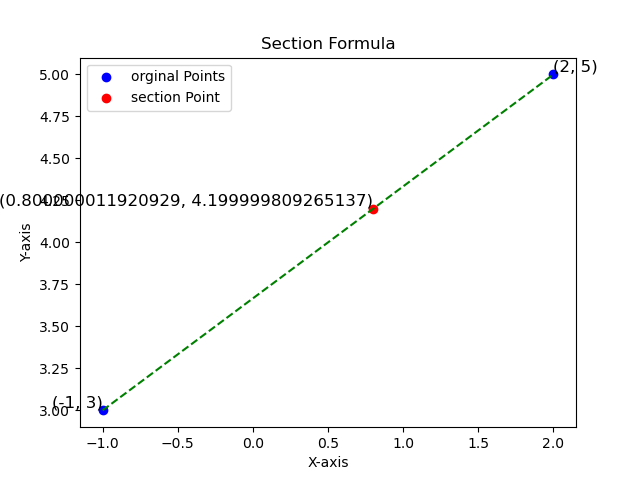
\includegraphics[width=0.7\linewidth]{figs/q1.png}
\label{fig1}
\end{figure}
\end{document}
